\begin{figure}[htbp]
  \centering
  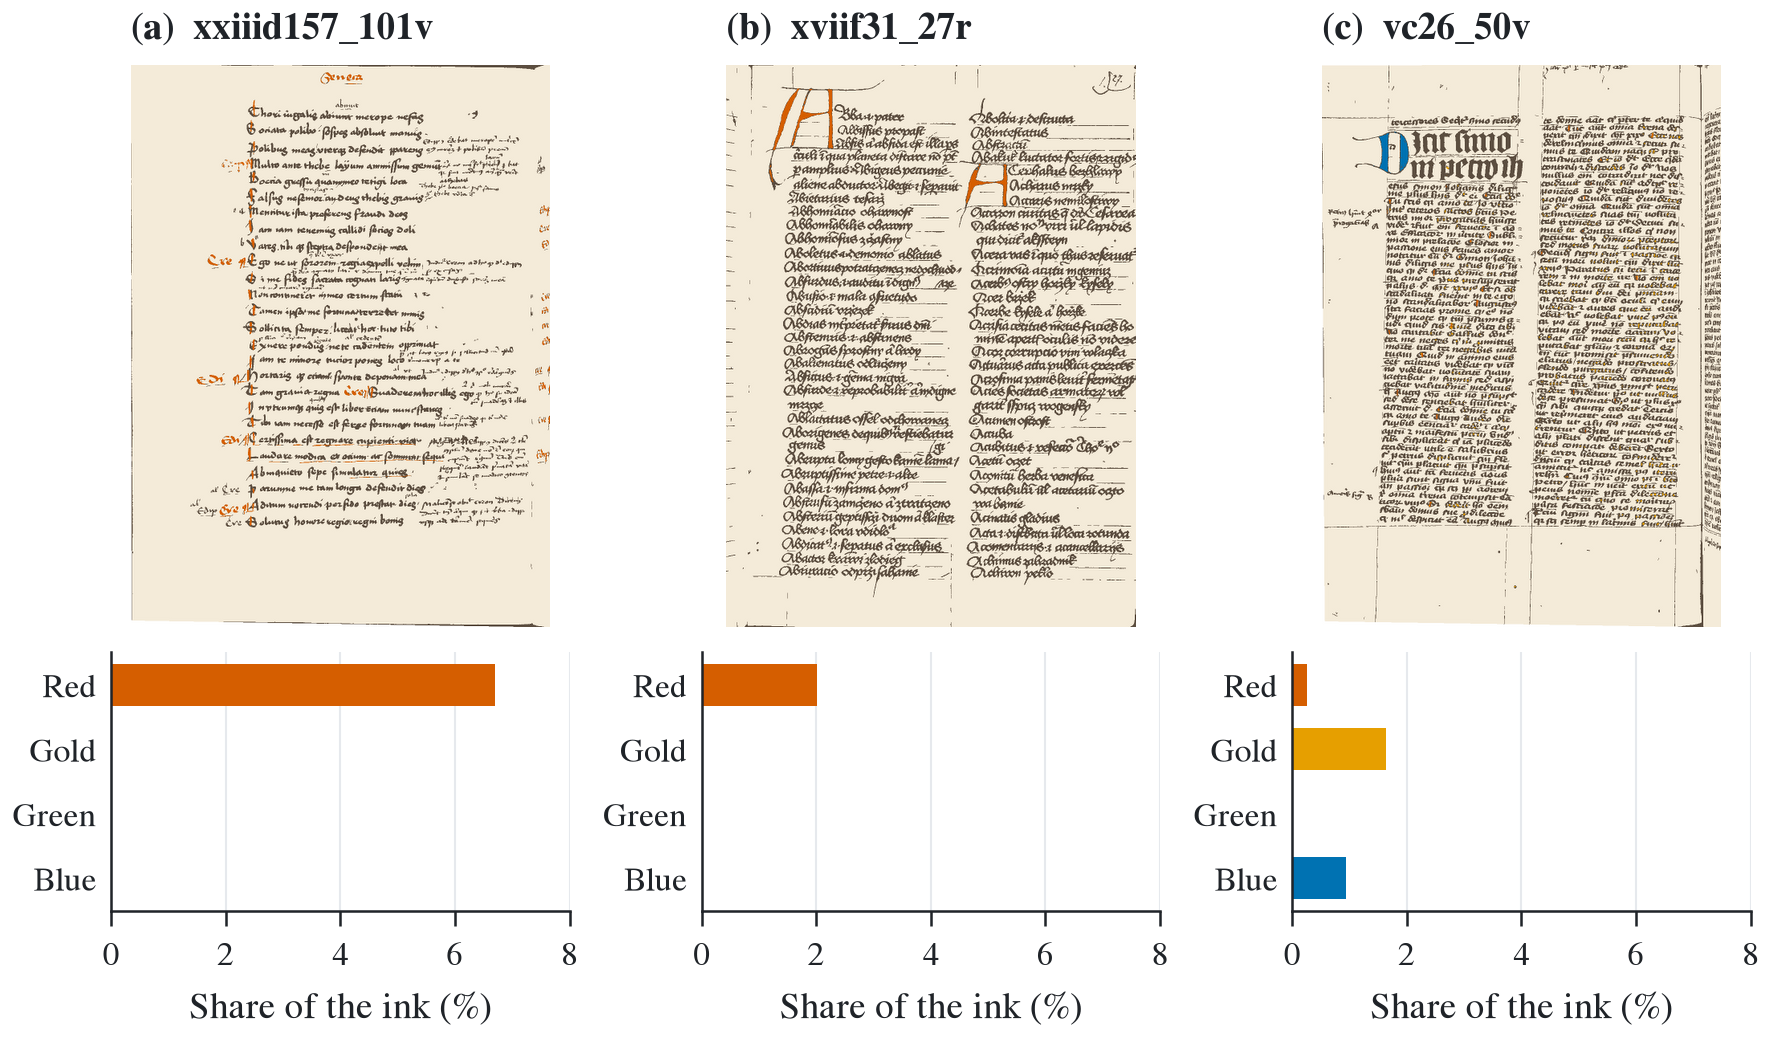
\includegraphics[width=15.00cm]{figures/ink_colour_on_page.png}
  \caption{Ink colour on three pages: each page's ink as the colour measures see it, the parchment made neutral (plain ink brown, chromatic ink, of chroma at least 25, in the colour of its hue class: red, gold, green or blue), beside the classes' shares of the ink. (a) xxiiid157\_101v: 6.7\% of the ink chromatic (red 6.7\%), 1.01 bits of hue entropy, 15\% rubric lines, 0 coloured initials; (b) xviif31\_27r: 2.0\% of the ink chromatic (red 2.0\%), 0.77 bits of hue entropy, 0\% rubric lines, 1 coloured initials; (c) vc26\_50v: 2.8\% of the ink chromatic (red 0.3\%, gold 1.6\%, blue 0.9\%), 1.83 bits of hue entropy, 0\% rubric lines, 1 coloured initials. Ink within stamps, left out of the measures, is light grey. Page images provided by Manuscriptorium (CC BY-NC 4.0).}
  \label{fig:ink_colour_on_page}
\end{figure}
